% Seminar 6: Modele VAR și cauzalitate Granger
% Prezentare academică de calitate Harvard
% Program de licență, Academia de Studii Economice din București

\documentclass[9pt, aspectratio=169, t]{beamer}

% Asigură încadrarea conținutului pe diapozitive
\setbeamersize{text margin left=8mm, text margin right=8mm}

%=============================================================================
% CONFIGURARE TEMĂ ȘI STIL
%=============================================================================
\usetheme{default}

% Color Palette (matching Redispatch PDF)
\definecolor{MainBlue}{RGB}{26, 58, 110}
\definecolor{AccentBlue}{RGB}{26, 58, 110}
\definecolor{IDAred}{RGB}{205, 0, 0}
\definecolor{DarkGray}{RGB}{51, 51, 51}
\definecolor{MediumGray}{RGB}{128, 128, 128}
\definecolor{LightGray}{RGB}{248, 248, 248}
\definecolor{VeryLightGray}{RGB}{235, 235, 235}
\definecolor{KeynoteGray}{RGB}{218, 218, 218}
\definecolor{SectionGray}{RGB}{120, 120, 120}
\definecolor{FooterGray}{RGB}{100, 100, 100}
\definecolor{Crimson}{RGB}{220, 53, 69}
\definecolor{Forest}{RGB}{46, 125, 50}
\definecolor{Amber}{RGB}{181, 133, 63}
\definecolor{Orange}{RGB}{230, 126, 34}
\definecolor{Purple}{RGB}{142, 68, 173}

% Gradient background (exact Keynote 315 gradient: white to RGB 218,218,218)
\setbeamertemplate{background}{%
    \begin{tikzpicture}[remember picture, overlay]
        \shade[shading=axis, shading angle=315,
        top color=white, bottom color=KeynoteGray]
        (current page.south west) rectangle (current page.north east);
    \end{tikzpicture}%
}
% Fallback solid color for compatibility
\setbeamercolor{background canvas}{bg=}

\setbeamercolor{palette primary}{bg=MainBlue, fg=white}
\setbeamercolor{palette secondary}{bg=MainBlue!85, fg=white}
\setbeamercolor{palette tertiary}{bg=MainBlue!70, fg=white}
\setbeamercolor{structure}{fg=MainBlue}
\setbeamercolor{title}{fg=IDAred}
\setbeamercolor{frametitle}{fg=IDAred, bg=}
\setbeamercolor{block title}{bg=MainBlue, fg=white}
\setbeamercolor{block body}{bg=VeryLightGray, fg=DarkGray}
\setbeamercolor{block title alerted}{bg=Crimson, fg=white}
\setbeamercolor{block body alerted}{bg=Crimson!8, fg=DarkGray}
\setbeamercolor{block title example}{bg=Forest, fg=white}
\setbeamercolor{block body example}{bg=Forest!8, fg=DarkGray}
\setbeamercolor{item}{fg=MainBlue}

% Footer colors (override Madrid theme blue)
\setbeamercolor{author in head/foot}{fg=FooterGray, bg=}
\setbeamercolor{title in head/foot}{fg=FooterGray, bg=}
\setbeamercolor{date in head/foot}{fg=FooterGray, bg=}
\setbeamercolor{section in head/foot}{fg=FooterGray, bg=}
\setbeamercolor{subsection in head/foot}{fg=FooterGray, bg=}

% Bullet styles (apply everywhere including blocks)
\setbeamertemplate{itemize item}{\color{MainBlue}$\boxdot$}
\setbeamertemplate{itemize subitem}{\color{MainBlue}$\blacktriangleright$}
\setbeamertemplate{itemize subsubitem}{\color{MainBlue}\tiny$\bullet$}
\setbeamertemplate{itemize/enumerate body begin}{\normalsize}
\setbeamertemplate{itemize/enumerate subbody begin}{\normalsize}

% Item spacing - compact style
\setlength{\leftmargini}{10pt}       % Level 1: minimal indent
\setlength{\leftmarginii}{10pt}      % Level 2: minimal additional indent
% Compact list spacing (zero extra space before/after lists in blocks)
\makeatletter
\def\@listi{\leftmargin\leftmargini \topsep 0pt \parsep 0pt \itemsep 0pt}
\def\@listii{\leftmargin\leftmarginii \topsep 0pt \parsep 0pt \itemsep 0pt}
\makeatother

\setbeamertemplate{navigation symbols}{}

%=============================================================================
% CUSTOM HEADLINE
%=============================================================================
\setbeamertemplate{headline}{%
    \vskip10pt%
    \hbox to \paperwidth{%
        \hskip0.5cm%
        {\small\color{FooterGray}\renewcommand{\hyperlink}[2]{##2}\insertsectionhead}%
        \hfill%
        \textcolor{FooterGray}{\small\insertframenumber}%
        \hskip0.5cm%
    }%
    \vskip4pt%
    {\color{FooterGray}\hrule height 0.4pt}%
}

%=============================================================================
% CUSTOM FOOTER
%=============================================================================
\usepackage{fontawesome5}

\setbeamertemplate{footline}{%
    {\color{FooterGray}\hrule height 0.4pt}%
    \vskip4pt%
    \hbox to \paperwidth{%
        \hskip0.5cm%
        \textcolor{FooterGray}{\small Analiza și Prognoza seriilor de timp}%
        \hfill%
        \raisebox{-0.1em}{%
            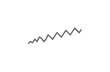
\begin{tikzpicture}[x=0.08em, y=0.08em, line width=0.4pt]
                \draw[FooterGray] (0,3) -- (1,4) -- (2,3.5) -- (3,5) -- (4,4) -- (5,6) -- (6,5.5) -- (7,4) -- (8,5) -- (9,7) -- (10,6) -- (11,5) -- (12,6.5) -- (13,8) -- (14,7) -- (15,6) -- (16,7.5) -- (17,9) -- (18,8) -- (19,7) -- (20,8.5) -- (21,10) -- (22,9) -- (23,8) -- (24,9.5);
            \end{tikzpicture}%
        }%
        \hskip0.5cm%
    }%
    \vskip6pt%
}

%=============================================================================
% PACHETE
%=============================================================================
\usepackage[utf8]{inputenc}
\usepackage[T1]{fontenc}
\usepackage[romanian]{babel}
\usepackage{amsmath, amssymb, amsthm}
\usepackage{mathtools}
\usepackage{bm}
\usepackage{tikz}
\usetikzlibrary{arrows.meta, positioning, shapes, calc, decorations.pathreplacing, shadings}
\usepackage{booktabs}
\usepackage{multirow}
\usepackage{array}
\usepackage{graphicx}
\usepackage{hyperref}
\usepackage{colortbl}
\hypersetup{colorlinks=true, linkcolor=MainBlue, urlcolor=MainBlue}
\graphicspath{{../../logos/}{../../charts/}}
\hfuzz=2pt  % Suppress tiny overfull warnings (<2pt)
\vfuzz=2pt  % Suppress tiny vertical overfull warnings (<2pt)

%=============================================================================
% COMANDA QUANTLET
%=============================================================================
\newcommand{\quantlet}[2]{%
    \hfill\href{#2}{%
        \raisebox{-0.15em}{\includegraphics[height=0.7em]{ql_logo.png}}%
        \textcolor{MainBlue}{\tiny\ #1}%
    }%
}

%=============================================================================
% COMENZI PERSONALIZATE
%=============================================================================
\newcommand{\E}{\mathbb{E}}
\newcommand{\Var}{\text{Var}}
\newcommand{\Cov}{\text{Cov}}
\newcommand{\Corr}{\text{Corr}}
\newcommand{\R}{\mathbb{R}}
\newcommand{\RMSE}{\text{RMSE}}
\newcommand{\MAE}{\text{MAE}}
\newcommand{\MAPE}{\text{MAPE}}
% Bold math commands for VAR models
\newcommand{\bY}{\mathbf{Y}}
\newcommand{\bX}{\mathbf{X}}
\newcommand{\bA}{\mathbf{A}}
\newcommand{\bB}{\mathbf{B}}
\newcommand{\bC}{\mathbf{C}}
\newcommand{\bc}{\mathbf{c}}
\newcommand{\bvarepsilon}{\boldsymbol{\varepsilon}}
\newcommand{\bepsilon}{\boldsymbol{\varepsilon}}
\newcommand{\bSigma}{\boldsymbol{\Sigma}}

\newcommand{\correct}{\textcolor{Forest}{\checkmark}}
\newcommand{\incorrect}{\textcolor{Crimson}{\texttimes}}

%=============================================================================
% PAGINA TITLU PERSONALIZATA
%=============================================================================
\defbeamertemplate*{title page}{hybrid}[1][]
{
    \vspace{0.2cm}
    \begin{center}
        \href{https://www.ase.ro}{\includegraphics[height=1.0cm]{ase_logo.png}}\hspace{0.3cm}%
        \href{https://theida.net}{\includegraphics[height=1.0cm]{ida_logo.png}}\hspace{0.3cm}%
        \href{https://blockchain-research-center.com}{\includegraphics[height=1.0cm]{brc_logo.png}}\hspace{0.3cm}%
        \href{https://www.ai4efin.ase.ro}{\includegraphics[height=1.0cm]{ai4efin_logo.png}}\hspace{0.3cm}%
        \href{https://ipe.ro/new}{\includegraphics[height=1.0cm]{acad_logo.png}}\hspace{0.3cm}%
        \href{https://www.digital-finance-msca.com}{\includegraphics[height=1.0cm]{msca_logo.png}}%
    \end{center}

    \vspace{0.6cm}

    \begin{center}
        \begin{minipage}{0.1\textwidth}
            \centering
            \href{https://quantlet.com}{\includegraphics[height=1.1cm]{ql_logo.png}}
        \end{minipage}%
        \begin{minipage}{0.78\textwidth}
            \centering
            {\LARGE\bfseries\usebeamercolor[fg]{title}\inserttitle}

            \vspace{0.3cm}

            {\usebeamerfont{subtitle}\usebeamercolor[fg]{title}\insertsubtitle}
        \end{minipage}%
        \begin{minipage}{0.1\textwidth}
            \centering
            \href{https://quantinar.com}{\includegraphics[height=1.1cm]{qr_logo.png}}
        \end{minipage}
    \end{center}

    \vspace{0.6cm}

    \hspace{0.5cm}{\usebeamerfont{author}\insertauthor}

    \vspace{0.3cm}

    \hspace{0.5cm}\begin{minipage}[t]{0.9\textwidth}
        \raggedright\small\insertinstitute
    \end{minipage}
}

%=============================================================================
% INFORMATII TITLU
%=============================================================================
\title[Analiza Seriilor de Timp]{Analiza și Prognoza seriilor de timp}
\subtitle{Seminar 6: Modele VAR și cauzalitate Granger}
\author[D.T. Pele]{Daniel Traian PELE}
\institute{Academia de Studii Economice din București\\
IDA Institute Digital Assets\\
Blockchain Research Center\\
AI4EFin Artificial Intelligence for Energy Finance\\
Academia Română, Institutul de Prognoză Economică\\
MSCA Digital Finance}
\date{}

\begin{document}

% Title page (no header/footer)
{
\setbeamertemplate{headline}{}
\setbeamertemplate{footline}{}
\begin{frame}
    \titlepage
\end{frame}
}

%=============================================================================
% OUTLINE
%=============================================================================
\begin{frame}{Cuprins Seminar}
    \tableofcontents
\end{frame}

%=============================================================================
% SECTION 1: REVIEW QUIZ
%=============================================================================
\section{Test de Recapitulare}

\begin{frame}{Test 1: Definiția VAR}
    \begin{alertblock}{Întrebare}
        Într-un model VAR(2) cu 3 variabile, câte matrice de coeficienți $\bA_i$ există?
    \end{alertblock}

    \vspace{0.3cm}

    \begin{block}{Variante de răspuns}
        \textcolor{MainBlue}{\textbf{(A)}} 2 \qquad
{indent}    \textcolor{MainBlue}{\textbf{(B)}} 3 \qquad
{indent}    \textcolor{MainBlue}{\textbf{(C)}} 6 \qquad
{indent}    \textcolor{MainBlue}{\textbf{(D)}} 9
    \end{block}

    \vspace{0.5cm}
    \begin{flushright}\textit{Răspunsul pe slide-ul următor...}\end{flushright}
\end{frame}

\begin{frame}{Test 1: Răspuns}
    \begin{exampleblock}{Răspuns: A -- 2 matrice de coeficienți}
        \textbf{Modelul VAR($p$)}: $\bY_t = \bc + \bA_1\bY_{t-1} + \bA_2\bY_{t-2} + \cdots + \bA_p\bY_{t-p} + \bvarepsilon_t$

        \vspace{0.3cm}
        \textbf{VAR(2) cu $K=3$}:
        \[
        \begin{pmatrix} Y_{1t} \\ Y_{2t} \\ Y_{3t} \end{pmatrix} = \bc + \underbrace{\bA_1}_{3\times 3}\begin{pmatrix} Y_{1,t-1} \\ Y_{2,t-1} \\ Y_{3,t-1} \end{pmatrix} + \underbrace{\bA_2}_{3\times 3}\begin{pmatrix} Y_{1,t-2} \\ Y_{2,t-2} \\ Y_{3,t-2} \end{pmatrix} + \bvarepsilon_t
        \]

        \textbf{Cheie}: $p$ = numărul de lag-uri = numărul de matrice
    \end{exampleblock}
\end{frame}

\begin{frame}{Test 2: Numărul de Parametri}
    \begin{alertblock}{Întrebare}
        Un VAR(2) cu $K=3$ variabile (incluzând constantele) are câți parametri de estimat per ecuație?
    \end{alertblock}

    \vspace{0.3cm}

    \begin{block}{Variante de răspuns}
        \textcolor{MainBlue}{\textbf{(A)}} 3 \qquad
{indent}    \textcolor{MainBlue}{\textbf{(B)}} 6 \qquad
{indent}    \textcolor{MainBlue}{\textbf{(C)}} 7 \qquad
{indent}    \textcolor{MainBlue}{\textbf{(D)}} 9
    \end{block}

    \vspace{0.5cm}
    \begin{flushright}\textit{Răspunsul pe slide-ul următor...}\end{flushright}
\end{frame}

\begin{frame}{Test 2: Răspuns}
    \begin{exampleblock}{Răspuns: C -- 7 parametri per ecuație}
        \begin{center}
            \includegraphics[width=0.95\textwidth, height=0.55\textheight, keepaspectratio]{sem5_var_parameters.pdf}
        \end{center}
        \vspace{-0.2cm}
        {\footnotesize
        \textbf{Formula}: Per ecuație = $1 + K \times p = 1 + 3 \times 2 = 7$. \textbf{Total}: $K(1 + Kp) = 3(1 + 6) = 21$ parametri
        }
    \end{exampleblock}
\end{frame}

\begin{frame}{Test 3: Cauzalitate Granger}
    \begin{alertblock}{Întrebare}
        ``$X$ cauzează Granger $Y$'' înseamnă:
    \end{alertblock}

    \vspace{0.3cm}

    \begin{block}{Variante de răspuns}
        \textcolor{MainBlue}{\textbf{(A)}} $X$ este cauza economică a lui $Y$\\[3pt]
        \textcolor{MainBlue}{\textbf{(B)}} Trecutul lui $X$ ajută la predicția lui $Y$\\[3pt]
        \textcolor{MainBlue}{\textbf{(C)}} $X$ și $Y$ sunt corelate contemporan\\[3pt]
        \textcolor{MainBlue}{\textbf{(D)}} $X$ crește întotdeauna când $Y$ crește
    \end{block}

    \vspace{0.5cm}
    \begin{flushright}\textit{Răspunsul pe slide-ul următor...}\end{flushright}
\end{frame}

\begin{frame}{Test 3: Răspuns}
    \begin{exampleblock}{Răspuns: B -- Trecutul lui $X$ ajută la predicția lui $Y$}
        \begin{center}
            \includegraphics[width=0.9\textwidth, height=0.55\textheight, keepaspectratio]{sem5_granger_diagram.pdf}
        \end{center}
        \vspace{-0.2cm}
        {\footnotesize
        \textbf{Cheie}: Relație predictivă, NU cauzalitate adevărată!
        }
    \end{exampleblock}
\end{frame}

\begin{frame}{Test 4: Testul de Cauzalitate Granger}
    \begin{alertblock}{Întrebare}
        Pentru a testa dacă $Y_2$ cauzează Granger $Y_1$ într-un VAR(p), testăm:
    \end{alertblock}

    \vspace{0.3cm}

    \begin{block}{Variante de răspuns}
        \textcolor{MainBlue}{\textbf{(A)}} Toți coeficienții din ecuația lui $Y_1$ sunt egali cu zero\\[3pt]
        \textcolor{MainBlue}{\textbf{(B)}} Coeficienții pe $Y_2$ întârziat din ecuația lui $Y_1$ sunt egali cu zero\\[3pt]
        \textcolor{MainBlue}{\textbf{(C)}} Coeficienții pe $Y_1$ întârziat din ecuația lui $Y_2$ sunt egali cu zero\\[3pt]
        \textcolor{MainBlue}{\textbf{(D)}} Covarianța erorilor este egală cu zero
    \end{block}

    \vspace{0.5cm}
    \begin{flushright}\textit{Răspunsul pe slide-ul următor...}\end{flushright}
\end{frame}

\begin{frame}{Test 4: Răspuns}
    \begin{exampleblock}{Răspuns: B -- Coeficienții pe $Y_2$ întârziat din ecuația lui $Y_1$ = 0}
        \textbf{Ipoteza nulă}: $H_0: a_{12}^{(1)} = a_{12}^{(2)} = \cdots = a_{12}^{(p)} = 0$

        \vspace{0.2cm}
        \textbf{Statistica de test}: Test Wald sau F cu $p$ restricții

        \vspace{0.2cm}
        \textbf{Interpretare}:
        \begin{itemize}
            \item Respingem $H_0$: $Y_2$ cauzează Granger $Y_1$
            \item Nu respingem: Fără evidență de relație predictivă
        \end{itemize}

        \vspace{0.2cm}
        \textbf{Notă}: Testați $Y_1 \to Y_2$ separat (coeficienți diferiți în ecuația lui $Y_2$)
    \end{exampleblock}
\end{frame}

\begin{frame}{Test 5: Stabilitatea VAR}
    \begin{alertblock}{Întrebare}
        Un model VAR(1) este stabil (staționar) dacă:
    \end{alertblock}

    \vspace{0.3cm}

    \begin{block}{Variante de răspuns}
        \textcolor{MainBlue}{\textbf{(A)}} Toate elementele diagonale ale lui $\bA_1$ sunt mai mici decât 1\\[3pt]
        \textcolor{MainBlue}{\textbf{(B)}} Determinantul lui $\bA_1$ este mai mic decât 1\\[3pt]
        \textcolor{MainBlue}{\textbf{(C)}} Toate valorile proprii ale lui $\bA_1$ sunt mai mici decât 1 în valoare absolută\\[3pt]
        \textcolor{MainBlue}{\textbf{(D)}} Urma lui $\bA_1$ este egală cu zero
    \end{block}

    \vspace{0.5cm}
    \begin{flushright}\textit{Răspunsul pe slide-ul următor...}\end{flushright}
\end{frame}

\begin{frame}{Test 5: Răspuns}
    \begin{exampleblock}{Răspuns: C -- Toate valorile proprii ale lui $\bA_1$ în interiorul cercului unitate}
        \begin{center}
            \includegraphics[width=0.95\textwidth, height=0.6\textheight, keepaspectratio]{sem5_var_stability.pdf}
        \end{center}
        \vspace{-0.2cm}
        {\footnotesize
        \textbf{Stabil}: Toate $|\lambda_i| < 1$ (în interiorul cercului unitate) $\Rightarrow$ șocurile dispar în timp
        }
    \end{exampleblock}
\end{frame}

\begin{frame}{Test 6: Funcții de Răspuns la Impuls}
    \begin{alertblock}{Întrebare}
        O funcție de răspuns la impuls arată:
    \end{alertblock}

    \vspace{0.3cm}

    \begin{block}{Variante de răspuns}
        \textcolor{MainBlue}{\textbf{(A)}} Corelația între două variabile\\[3pt]
        \textcolor{MainBlue}{\textbf{(B)}} Efectul unui șoc la o variabilă asupra tuturor variabilelor în timp\\[3pt]
        \textcolor{MainBlue}{\textbf{(C)}} Acuratețea prognozei modelului\\[3pt]
        \textcolor{MainBlue}{\textbf{(D)}} Valorile-p ale testelor de coeficienți
    \end{block}

    \vspace{0.5cm}
    \begin{flushright}\textit{Răspunsul pe slide-ul următor...}\end{flushright}
\end{frame}

\begin{frame}{Test 6: Răspuns}
    \begin{exampleblock}{Răspuns: B -- Efectul șocului asupra tuturor variabilelor în timp}
        \begin{center}
            \includegraphics[width=0.95\textwidth, height=0.6\textheight, keepaspectratio]{sem5_irf_example.pdf}
        \end{center}
        \vspace{-0.2cm}
        {\footnotesize
        \textbf{IRF}$_{ij}(h)$: Răspunsul variabilei $i$ la orizontul $h$ la șocul în variabila $j$
        }
    \end{exampleblock}
\end{frame}

\begin{frame}{Test 7: Selectarea Ordinului Lag}
    \begin{alertblock}{Întrebare}
        Care criteriu selectează de obicei cel mai simplu model VAR?
    \end{alertblock}

    \vspace{0.3cm}

    \begin{block}{Variante de răspuns}
        \textcolor{MainBlue}{\textbf{(A)}} AIC (Criteriul Informațional Akaike)\\[3pt]
        \textcolor{MainBlue}{\textbf{(B)}} BIC (Criteriul Informațional Bayesian)\\[3pt]
        \textcolor{MainBlue}{\textbf{(C)}} FPE (Eroarea Finală de Predicție)\\[3pt]
        \textcolor{MainBlue}{\textbf{(D)}} $R^2$ ajustat
    \end{block}

    \vspace{0.5cm}
    \begin{flushright}\textit{Răspunsul pe slide-ul următor...}\end{flushright}
\end{frame}

\begin{frame}{Test 7: Răspuns}
    \begin{exampleblock}{Răspuns: B -- BIC (Criteriul Informațional Bayesian)}
        \textbf{Comparația penalizărilor}:
        \begin{itemize}
            \item AIC: $-2\ln L + 2k$
            \item BIC: $-2\ln L + k\ln n$
            \item[] {\scriptsize $L$ = maximul funcției de verosimilitate, $k$ = nr.\ parametri, $n$ = dimensiunea eșantionului}
        \end{itemize}

        Deoarece $\ln n > 2$ pentru $n > 8$, BIC penalizează complexitatea mai puternic

        \vspace{0.2cm}
        \textbf{Îndrumări practice}:
        \begin{itemize}
            \item Prognoză: AIC poate performa mai bine
            \item Inferență/parsimonie: BIC preferat
            \item Eșantioane mari: BIC consistent, AIC tinde să supraajusteze
        \end{itemize}
    \end{exampleblock}
\end{frame}

\begin{frame}{Test 8: interpretarea Cauzalității Granger}
    \begin{alertblock}{Întrebare}
        ``$X$ cauzează Granger $Y$'' înseamnă:
    \end{alertblock}

    \vspace{0.3cm}

    \begin{block}{Variante de răspuns}
        \textcolor{MainBlue}{\textbf{(A)}} $X$ este cauza adevărată a lui $Y$\\[3pt]
        \textcolor{MainBlue}{\textbf{(B)}} Valorile trecute ale lui $X$ ajută la predicția lui $Y$ dincolo de trecutul propriu al lui $Y$\\[3pt]
        \textcolor{MainBlue}{\textbf{(C)}} $X$ și $Y$ sunt corelate\\[3pt]
        \textcolor{MainBlue}{\textbf{(D)}} $Y$ depinde doar de $X$
    \end{block}

    \vspace{0.5cm}
    \begin{flushright}\textit{Răspunsul pe slide-ul următor...}\end{flushright}
\end{frame}

\begin{frame}{Test 8: Răspuns}
    \begin{exampleblock}{Răspuns: B}
        Cauzalitatea Granger se referă la conținutul \textbf{predictiv}, nu la cauzalitatea adevărată. $X$ cauzează Granger $Y$ dacă termenii lui $X$ întârziați sunt semnificativi conjunct în ecuația lui $Y$, după controlul pentru $Y$ întârziat.
    \end{exampleblock}
\end{frame}

\begin{frame}{Test 9: Descompunerea varianței Erorii de Prognoză}
    \begin{alertblock}{Întrebare}
        FEVD (Descompunerea varianței Erorii de Prognoză) ne spune:
    \end{alertblock}

    \vspace{0.3cm}

    \begin{block}{Variante de răspuns}
        \textcolor{MainBlue}{\textbf{(A)}} Corelația între variabile\\[3pt]
        \textcolor{MainBlue}{\textbf{(B)}} Ce proporție din varianța erorii de prognoză vine din fiecare șoc\\[3pt]
        \textcolor{MainBlue}{\textbf{(C)}} Orizontul optim de prognoză\\[3pt]
        \textcolor{MainBlue}{\textbf{(D)}} Ce variabile să includem în model
    \end{block}

    \vspace{0.5cm}
    \begin{flushright}\textit{Răspunsul pe slide-ul următor...}\end{flushright}
\end{frame}

\begin{frame}{Test 9: Răspuns}
    \begin{exampleblock}{Răspuns: B -- Proporția varianței erorii de prognoză din fiecare șoc}
        \begin{center}
            \includegraphics[width=0.95\textwidth, height=0.6\textheight, keepaspectratio]{sem5_fevd_example.pdf}
        \end{center}
        \vspace{-0.2cm}
        {\footnotesize
        \textbf{FEVD}: Arată cât din incertitudinea prognozei vine din fiecare șoc la diferite orizonturi
        }
    \end{exampleblock}
\end{frame}

\begin{frame}{Test 10: VAR Structural vs Forma Redusă}
    \begin{alertblock}{Întrebare}
        Diferența dintre VAR structural (SVAR) și VAR forma redusă este:
    \end{alertblock}

    \vspace{0.3cm}

    \begin{block}{Variante de răspuns}
        \textcolor{MainBlue}{\textbf{(A)}} SVAR are mai multe variabile\\[3pt]
        \textcolor{MainBlue}{\textbf{(B)}} SVAR permite efecte contemporane între variabile\\[3pt]
        \textcolor{MainBlue}{\textbf{(C)}} SVAR folosește metode de estimare diferite\\[3pt]
        \textcolor{MainBlue}{\textbf{(D)}} Nu există diferență
    \end{block}

    \vspace{0.5cm}
    \begin{flushright}\textit{Răspunsul pe slide-ul următor...}\end{flushright}
\end{frame}

\begin{frame}{Test 10: Răspuns}
    \begin{exampleblock}{Răspuns: B}
        VAR forma redusă: șocurile sunt corelate, fără efecte contemporane în ecuații. SVAR: impune restricții de identificare pentru a recupera șocuri structurale cu interpretare economică (de ex., șoc de politică monetară).
    \end{exampleblock}
\end{frame}

\begin{frame}{Test 11: Descompunerea Cholesky}
    \begin{alertblock}{Întrebare}
        Ordonarea Cholesky în analiza IRF presupune:
    \end{alertblock}

    \vspace{0.3cm}

    \begin{block}{Variante de răspuns}
        \textcolor{MainBlue}{\textbf{(A)}} Toate variabilele sunt la fel de importante\\[3pt]
        \textcolor{MainBlue}{\textbf{(B)}} Variabilele ordonate primele afectează contemporan variabilele de mai târziu, nu invers\\[3pt]
        \textcolor{MainBlue}{\textbf{(C)}} Șocurile sunt necorelate\\[3pt]
        \textcolor{MainBlue}{\textbf{(D)}} Nu sunt necesare restricții
    \end{block}

    \vspace{0.5cm}
    \begin{flushright}\textit{Răspunsul pe slide-ul următor...}\end{flushright}
\end{frame}

\begin{frame}{Test 11: Răspuns}
    \begin{exampleblock}{Răspuns: B -- Variabilele ordonate primele afectează contemporan pe cele de mai târziu}
        \begin{center}
            \includegraphics[width=0.95\textwidth, height=0.6\textheight, keepaspectratio]{sem5_cholesky_ordering.pdf}
        \end{center}
        \vspace{-0.2cm}
        {\footnotesize
        \textbf{Cholesky}: Structură recursivă. Ordonarea contează -- justificați prin teoria economică (cel mai exogen primul)!
        }
    \end{exampleblock}
\end{frame}

\begin{frame}{Test 12: Diagnosticele Reziduurilor VAR}
    \begin{alertblock}{Întrebare}
        Într-un VAR bine specificat, reziduurile ar trebui să fie:
    \end{alertblock}

    \vspace{0.3cm}

    \begin{block}{Variante de răspuns}
        \textcolor{MainBlue}{\textbf{(A)}} Autocorelate dar homoscedastice\\[3pt]
        \textcolor{MainBlue}{\textbf{(B)}} Zgomot alb (fără autocorelație)\\[3pt]
        \textcolor{MainBlue}{\textbf{(C)}} Doar distribuite normal\\[3pt]
        \textcolor{MainBlue}{\textbf{(D)}} Corelate între ecuații
    \end{block}

    \vspace{0.5cm}
    \begin{flushright}\textit{Răspunsul pe slide-ul următor...}\end{flushright}
\end{frame}

\begin{frame}{Test 12: Răspuns}
    \begin{exampleblock}{Răspuns: B -- Zgomot alb (fără autocorelație)}
        \begin{center}
            \includegraphics[width=0.95\textwidth, height=0.6\textheight, keepaspectratio]{sem5_var_diagnostics.pdf}
        \end{center}
        \vspace{-0.2cm}
        {\footnotesize
        \textbf{Diagnostice}: Reziduurile ar trebui să fie zgomot alb. Folosiți testul Portmanteau/LM. Corelația între ecuații este permisă ($\Sigma_u$).
        }
    \end{exampleblock}
\end{frame}

\begin{frame}{Test 13: Cointegrare și VAR}
    \begin{alertblock}{Întrebare}
        Dacă variabilele sunt I(1) și cointegrate, ar trebui să folosiți:
    \end{alertblock}

    \vspace{0.3cm}

    \begin{block}{Variante de răspuns}
        \textcolor{MainBlue}{\textbf{(A)}} VAR în niveluri\\[3pt]
        \textcolor{MainBlue}{\textbf{(B)}} VAR în prime diferențe\\[3pt]
        \textcolor{MainBlue}{\textbf{(C)}} Model cu Corecție a Erorilor Vectoriale (VECM)\\[3pt]
        \textcolor{MainBlue}{\textbf{(D)}} Modele ARIMA univariate
    \end{block}

    \vspace{0.5cm}
    \begin{flushright}\textit{Răspunsul pe slide-ul următor...}\end{flushright}
\end{frame}

\begin{frame}{Test 13: Răspuns}
    \begin{exampleblock}{Răspuns: C}
        Cu cointegrare, VAR în diferențe pierde informația pe termen lung, în timp ce VAR în niveluri poate fi ineficient. VECM încorporează atât dinamica pe termen scurt cât și relațiile de echilibru pe termen lung prin termenul de corecție a erorilor.
    \end{exampleblock}
\end{frame}

\begin{frame}{Test 14: Cauzalitate Instantanee}
    \begin{alertblock}{Întrebare}
        Cauzalitatea instantanee diferă de cauzalitatea Granger deoarece testează:
    \end{alertblock}

    \vspace{0.3cm}

    \begin{block}{Variante de răspuns}
        \textcolor{MainBlue}{\textbf{(A)}} Doar relații întârziate\\[3pt]
        \textcolor{MainBlue}{\textbf{(B)}} Corelația contemporană a reziduurilor\\[3pt]
        \textcolor{MainBlue}{\textbf{(C)}} Relații pe termen lung\\[3pt]
        \textcolor{MainBlue}{\textbf{(D)}} Stabilitatea modelului
    \end{block}

    \vspace{0.5cm}
    \begin{flushright}\textit{Răspunsul pe slide-ul următor...}\end{flushright}
\end{frame}

\begin{frame}{Test 14: Răspuns}
    \begin{exampleblock}{Răspuns: B}
        Cauzalitatea instantanee testează dacă șocurile la $X$ și $Y$ sunt corelate în aceeași perioadă (corelația reziduurilor VAR). Cauzalitatea Granger testează dacă valorile \textit{întârziate} ajută la predicție.
    \end{exampleblock}
\end{frame}

%=============================================================================
% TRUE/FALSE QUESTIONS
%=============================================================================
\section{Întrebări Adevărat/Fals}

\begin{frame}{Întrebări Adevărat/Fals}
    Determinați dacă fiecare afirmație este Adevărată sau Falsă:

    \vspace{0.3cm}
    \begin{enumerate}
        \item Modelele VAR tratează toate variabilele ca endogene.
        \item Cauzalitatea Granger dovedește cauzalitatea economică adevărată.
        \item Un VAR stabil are întotdeauna valorile proprii în interiorul cercului unitate.
        \item Rezultatele FEVD depind de ordonarea variabilelor.
        \item VAR poate fi estimat prin OLS ecuație cu ecuație.
        \item Răspunsurile la impuls dispar în cele din urmă într-un VAR stabil.
    \end{enumerate}

    \vspace{0.3cm}
    \begin{flushright}\textit{Răspunsurile pe slide-ul următor...}\end{flushright}
\end{frame}

\begin{frame}{Adevărat/Fals: Soluții}
    {\small
    \begin{enumerate}\setlength{\itemsep}{1pt}
        \item Modelele VAR tratează toate variabilele ca endogene. \hfill \textcolor{Forest}{\textbf{ADEVĂRAT}}

        {\footnotesize \textcolor{MediumGray}{Fiecare variabilă este regresată pe lag-urile tuturor variabilelor, inclusiv pe ea însăși.}}

        \item Cauzalitatea Granger dovedește cauzalitatea economică adevărată. \hfill \textcolor{Crimson}{\textbf{FALS}}

        {\footnotesize \textcolor{MediumGray}{Arată doar conținut predictiv, nu cauzalitate structurală.}}

        \item Un VAR stabil are întotdeauna valorile proprii în interiorul cercului unitate. \hfill \textcolor{Forest}{\textbf{ADEVĂRAT}}

        {\footnotesize \textcolor{MediumGray}{Condiția de stabilitate: toate valorile proprii ale matricei companion satisfac $|\lambda_i| < 1$.}}

        \item Rezultatele FEVD depind de ordonarea variabilelor. \hfill \textcolor{Forest}{\textbf{ADEVĂRAT}}

        {\footnotesize \textcolor{MediumGray}{Sub identificarea Cholesky, ordonări diferite dau rezultate diferite.}}

        \item VAR poate fi estimat prin OLS ecuație cu ecuație. \hfill \textcolor{Forest}{\textbf{ADEVĂRAT}}

        {\footnotesize \textcolor{MediumGray}{Cu aceiași regresori în fiecare ecuație, OLS = GLS = ML (sub normalitate).}}

        \item Răspunsurile la impuls dispar în cele din urmă într-un VAR stabil. \hfill \textcolor{Forest}{\textbf{ADEVĂRAT}}

        {\footnotesize \textcolor{MediumGray}{Stabilitatea asigură că șocurile au efecte tranzitorii; IRF $\to 0$ când $h \to \infty$.}}
    \end{enumerate}
    }
\end{frame}

%=============================================================================
% SECTION 2: PRACTICE PROBLEMS
%=============================================================================
\section{Probleme Practice}

\begin{frame}{Problema 1: Scrierea Ecuațiilor VAR}
    \begin{block}{Exercițiu}
        Scrieți cele două ecuații pentru un model VAR(1) bivariat cu variabilele $Y_t$ (creșterea PIB) și $X_t$ (inflația).
    \end{block}

    \vspace{0.5cm}
    \begin{flushright}\textit{Răspunsul pe slide-ul următor...}\end{flushright}
\end{frame}

\begin{frame}{Problema 1: Soluție}
    \begin{exampleblock}{Soluție}
        \begin{align*}
            Y_t &= c_1 + a_{11} Y_{t-1} + a_{12} X_{t-1} + \varepsilon_{1t} \\[0.2cm]
            X_t &= c_2 + a_{21} Y_{t-1} + a_{22} X_{t-1} + \varepsilon_{2t}
        \end{align*}

        \textbf{Interpretare}:
        \begin{itemize}
            \item $a_{12}$: Efectul inflației trecute asupra creșterii PIB curente
            \item $a_{21}$: Efectul creșterii PIB trecute asupra inflației curente
        \end{itemize}
    \end{exampleblock}
\end{frame}

\begin{frame}{Problema 2: Numărarea Parametrilor}
    \begin{block}{Exercițiu}
        Câți parametri totali trebuie estimați într-un VAR(3) cu $K=4$ variabile (incluzând constantele)?
    \end{block}

    \vspace{0.5cm}
    \begin{flushright}\textit{Răspunsul pe slide-ul următor...}\end{flushright}
\end{frame}

\begin{frame}{Problema 2: Soluție}
    \begin{exampleblock}{Soluție}
        Per ecuație: $1 + K \times p = 1 + 4 \times 3 = 13$ parametri

        \vspace{0.2cm}
        Total pentru $K=4$ ecuații: $4 \times 13 = \mathbf{52}$ parametri

        \vspace{0.2cm}
        Plus matricea de covarianță $\boldsymbol{\Sigma}$: $K(K+1)/2 = 4 \times 5 / 2 = 10$ elemente unice

        \vspace{0.2cm}
        \textbf{Total general: 62 parametri}

        \vspace{0.2cm}
        \textit{Acesta este motivul pentru care VAR-urile pot fi ``supraparametrizate'' cu date limitate!}
    \end{exampleblock}
\end{frame}

\begin{frame}{Problema 3: interpretarea Cauzalității Granger}
    \begin{block}{Exercițiu}
        Un test de cauzalitate Granger dă:
        \begin{itemize}\setlength{\itemsep}{0pt}
            \item $H_0$: Banii nu cauzează Granger PIB. valoare-p = 0.02
            \item $H_0$: PIB nu cauzează Granger Banii. valoare-p = 0.35
        \end{itemize}
        Interpretați aceste rezultate.
    \end{block}

    \vspace{0.5cm}
    \begin{flushright}\textit{Răspunsul pe slide-ul următor...}\end{flushright}
\end{frame}

\begin{frame}{Problema 3: Soluție}
    \begin{exampleblock}{Soluție}
        \begin{itemize}\setlength{\itemsep}{2pt}
            \item \textbf{Respingem} $H_0$ la 5\%: Banii \textbf{cauzează Granger} PIB
            \item \textbf{Nu respingem} $H_0$: PIB \textbf{nu} cauzează Granger Banii
        \end{itemize}

        \vspace{0.3cm}
        \textbf{Concluzie}: Cauzalitate unidirecțională: Bani $\rightarrow$ PIB

        \vspace{0.3cm}
        \textit{Interpretare}: Masa monetară trecută ajută la predicția creșterii PIB. Aceasta este consistentă cu punctele de vedere monetariste, dar amintiți-vă: cauzalitate Granger $\neq$ cauzalitate structurală!
    \end{exampleblock}
\end{frame}

\begin{frame}{Problema 4: Verificarea Stabilității}
    \begin{block}{Exercițiu}
        Pentru VAR(1) cu $\bA_1 = \begin{pmatrix} 0.7 & 0.2 \\ 0.1 & 0.5 \end{pmatrix}$, verificați stabilitatea.
    \end{block}

    \vspace{0.5cm}
    \begin{flushright}\textit{Răspunsul pe slide-ul următor...}\end{flushright}
\end{frame}

\begin{frame}{Problema 4: Soluție}
    \begin{exampleblock}{Soluție}
        Găsiți valorile proprii: $\det(\bA_1 - \lambda \mathbf{I}) = 0$

        $(0.7 - \lambda)(0.5 - \lambda) - (0.2)(0.1) = 0$

        $\lambda^2 - 1.2\lambda + 0.33 = 0$

        $\lambda = \frac{1.2 \pm \sqrt{1.44 - 1.32}}{2} = \frac{1.2 \pm 0.346}{2}$

        $\lambda_1 = 0.773, \quad \lambda_2 = 0.427$

        \vspace{0.3cm}
        Ambele $|\lambda_i| < 1$ $\Rightarrow$ \textbf{Stabil!}
    \end{exampleblock}
\end{frame}

\begin{frame}{Problema 5: Calculul IRF}
    \begin{block}{Exercițiu}
        Pentru VAR(1) cu $\bA = \begin{pmatrix} 0.5 & 0.2 \\ 0 & 0.6 \end{pmatrix}$, calculați $\boldsymbol{\Phi}_2$ (răspunsul la $h=2$).
    \end{block}

    \vspace{0.5cm}
    \begin{flushright}\textit{Răspunsul pe slide-ul următor...}\end{flushright}
\end{frame}

\begin{frame}{Problema 5: Soluție}
    \begin{exampleblock}{Soluție}
        $\boldsymbol{\Phi}_2 = \bA^2 = \begin{pmatrix} 0.5 & 0.2 \\ 0 & 0.6 \end{pmatrix} \begin{pmatrix} 0.5 & 0.2 \\ 0 & 0.6 \end{pmatrix}$

        \vspace{0.3cm}
        $= \begin{pmatrix} 0.25 + 0 & 0.10 + 0.12 \\ 0 + 0 & 0 + 0.36 \end{pmatrix} = \begin{pmatrix} 0.25 & 0.22 \\ 0 & 0.36 \end{pmatrix}$

        \vspace{0.3cm}
        \textbf{Interpretare}: Un șoc unitar la $Y_2$ la $t$ crește $Y_1$ cu 0.22 la $t+2$.
    \end{exampleblock}
\end{frame}

%=============================================================================
% SECTION 3: WORKED EXAMPLES
%=============================================================================
\section{Exemple Rezolvate}

\begin{frame}{Exemplu: Randamente de Acțiuni și Volum de Tranzacționare}
    {\small
    \begin{block}{Scenariu}
        Date zilnice despre randamentele acțiunilor ($R_t$) și volumul de tranzacționare ($V_t$). Testați cauzalitatea Granger în ambele direcții.
    \end{block}
    \begin{exampleblock}{Constatări Tipice în Literatura Financiară}
        \begin{itemize}\setlength{\itemsep}{0pt}
            \item Randamentele adesea cauzează Granger volumul (modificările de preț declanșează tranzacționare)
            \item Volumul uneori cauzează Granger randamentele (volumul ca indicator anticipator)
            \item Rezultate: Adesea cauzalitate \textbf{bidirecțională} $R \leftrightarrow V$
        \end{itemize}
    \end{exampleblock}
    \begin{block}{Problemă Practică}
        Randamentele acțiunilor sunt de obicei staționare, dar volumul poate necesita transformare (log sau diferențiere).
    \end{block}
    }
\end{frame}

\begin{frame}{Exemplu: Rate de Dobândă și Inflație}
    {\small
    \begin{block}{Contextul Regulii Taylor}
        Băncile centrale stabilesc ratele de dobândă ($i_t$) ca răspuns la inflație ($\pi_t$):
        $i_t = r^* + \pi^* + 1.5(\pi_t - \pi^*) + 0.5(y_t - y^*)$
    \end{block}
    \begin{exampleblock}{Întrebări de Analiză VAR}
        \begin{itemize}\setlength{\itemsep}{0pt}
            \item Inflația cauzează Granger ratele de dobândă? (Reacția băncii centrale)
            \item Ratele de dobândă cauzează Granger inflația? (Transmisia politicii monetare)
        \end{itemize}
    \end{exampleblock}
    \begin{block}{Rezultate Așteptate}
        Cauzalitate bidirecțională: $\pi \to i$ rapid (reacția politicii), $i \to \pi$ întârziat (efectul politicii)
    \end{block}
    }
\end{frame}

\begin{frame}{Analiza VAR în Python: Funcții Cheie}
    {\footnotesize
    \begin{block}{Biblioteci Esențiale}
        \texttt{from statsmodels.tsa.api import VAR} \\
        \texttt{from statsmodels.tsa.stattools import grangercausalitytests}
    \end{block}

    \begin{block}{flux de lucru}
        \begin{enumerate}\setlength{\itemsep}{0pt}
            \item Creați DataFrame: \texttt{data = pd.DataFrame(\{'pib': ..., 'somaj': ...\})}
            \item Ajustați VAR: \texttt{model = VAR(data); results = model.fit(maxlags=8, ic='aic')}
            \item Obțineți IRF: \texttt{irf = results.irf(periods=20)}
            \item Obțineți FEVD: \texttt{fevd = results.fevd(periods=20)}
            \item Teste Granger: \texttt{grangercausalitytests(data[['y', 'x']], maxlag=4)}
        \end{enumerate}
    \end{block}

    \begin{alertblock}{Notă}
        Exemple complete de lucru sunt furnizate în notebook-urile Jupyter.
    \end{alertblock}
    }
\end{frame}

%=============================================================================
% SECTION 4: REAL DATA ANALYSIS
%=============================================================================
\section{Analiză pe Date Reale}

\begin{frame}{Studiu de Caz: PIB și Șomaj}
    \vspace{0.3cm}
    \begin{center}
        \includegraphics[width=0.75\textwidth, height=0.38\textheight, keepaspectratio]{ch5_gdp_unemployment.pdf}
    \end{center}
    \vspace{-0.1cm}
    \begin{block}{Observații}
        \textbf{Sus}: Rata de creștere a PIB Real SUA (trimestrial). \textbf{Jos}: Rata șomajului SUA. Relație negativă clară (Legea lui Okun). Modelul VAR poate captura interacțiunile dinamice dintre aceste variabile.
    \end{block}
\end{frame}

\begin{frame}{Analiza Corelației Încrucișate}
    \vspace{0.3cm}
    \begin{center}
        \includegraphics[width=0.75\textwidth, height=0.38\textheight, keepaspectratio]{ch5_cross_correlation.pdf}
    \end{center}
    \vspace{-0.1cm}
    \begin{block}{Observații}
        Corelația încrucișată măsoară relațiile de anticipare-întârziere. Corelație negativă la lag 0: relație inversă contemporană. Model asimetric sugerează că șomajul răspunde la PIB cu întârziere. Ajută la informarea selectării ordinului lag VAR.
    \end{block}
\end{frame}

\begin{frame}{Vizual: Funcția de Corelație Încrucișată}
    \begin{center}
        \includegraphics[width=0.9\textwidth, height=0.65\textheight, keepaspectratio]{ch5_def_ccf.pdf}
    \end{center}
    \vspace{-0.3cm}
    {\small CCF măsoară corelația dintre două serii la lag-uri diferite, relevând relații de anticipare-întârziere.}
\end{frame}

\begin{frame}{Rezultate Estimare VAR}
    {\small
    \begin{block}{Model: VAR(2) pentru Creșterea PIB și Șomaj}
        \begin{center}
        \begin{tabular}{lcccc}
            \toprule
            \textbf{Ecuație} & \textbf{Variabilă} & \textbf{Coef.} & \textbf{Eroare Std.} & \textbf{t-stat} \\
            \midrule
            \multirow{4}{*}{$\Delta PIB_t$} & $\Delta PIB_{t-1}$ & $0.312$ & $0.087$ & $3.59$ \\
            & $\Delta PIB_{t-2}$ & $0.145$ & $0.082$ & $1.77$ \\
            & $U_{t-1}$ & $-0.421$ & $0.156$ & $-2.70$ \\
            & $U_{t-2}$ & $0.198$ & $0.148$ & $1.34$ \\
            \midrule
            \multirow{4}{*}{$U_t$} & $\Delta PIB_{t-1}$ & $-0.087$ & $0.032$ & $-2.72$ \\
            & $\Delta PIB_{t-2}$ & $-0.045$ & $0.030$ & $-1.50$ \\
            & $U_{t-1}$ & $1.456$ & $0.058$ & $25.1$ \\
            & $U_{t-2}$ & $-0.521$ & $0.055$ & $-9.47$ \\
            \bottomrule
        \end{tabular}
        \end{center}
    \end{block}
    }
\end{frame}

\begin{frame}{Funcții de Răspuns la Impuls}
    \vspace{0.3cm}
    \begin{center}
        \includegraphics[width=0.75\textwidth, height=0.38\textheight, keepaspectratio]{ch5_irf.pdf}
    \end{center}
    \vspace{-0.1cm}
    \begin{block}{Observații}
    {\small
        \begin{itemize}\setlength{\itemsep}{2pt}
            \item IRF arată răspunsul dinamic la șocuri de o unitate
            \item Șocul PIB: efect pozitiv temporar asupra PIB, negativ asupra șomajului
            \item Șocul șomajului: efect negativ asupra PIB, persistent asupra șomajului
            \item Benzile de încredere de 95\% arată incertitudinea în răspunsuri
        \end{itemize}
    }
    \end{block}
\end{frame}

\begin{frame}{Descompunerea varianței Erorii de Prognoză}
    \vspace{0.3cm}
    \begin{center}
        \includegraphics[width=0.75\textwidth, height=0.38\textheight, keepaspectratio]{ch5_fevd.pdf}
    \end{center}
    \vspace{-0.1cm}
    \begin{block}{Observații}
    {\small
        \begin{itemize}\setlength{\itemsep}{2pt}
            \item FEVD arată proporția varianței explicată de fiecare șoc
            \item Varianța PIB: explicată în mare parte de șocurile proprii, parțial de șomaj
            \item Varianța șomajului: foarte persistentă (șocurile proprii dominante)
            \item Oferă perspectivă asupra importanței relative a diferitelor șocuri
        \end{itemize}
    }
    \end{block}
\end{frame}

%=============================================================================
% SECTION 5: DISCUSSION TOPICS
%=============================================================================
\section{Subiecte de Discuție}

\begin{frame}{Discuție: Cauzalitate Granger vs Cauzalitate Adevărată}
    {\small
    \begin{alertblock}{Întrebare Cheie}
        Dacă $X$ cauzează Granger $Y$, înseamnă aceasta că $X$ cauzează de fapt $Y$? \textbf{NU!}
    \end{alertblock}
    \begin{block}{De ce Poate Eșua Cauzalitatea Granger}
        \begin{itemize}\setlength{\itemsep}{0pt}
            \item \textbf{Omiterea variabilelor}: $Z$ ar putea cauza atât $X$ cât și $Y$ (de ex., vremea $\to$ înghețată \& înecuri)
            \item \textbf{Efecte de anticipare}: Piețele anticipează evenimente viitoare (prețuri acțiuni $\to$ câștiguri)
            \item \textbf{Probleme de agregare}: Momentul colectării datelor contează
        \end{itemize}
    \end{block}
    \begin{exampleblock}{Concluzie}
        Cauzalitatea Granger se referă la \textbf{predicție}, nu la \textbf{mecanism}. Pentru cauzalitate structurală, este nevoie de teorie + strategie de identificare.
    \end{exampleblock}
    }
\end{frame}

\begin{frame}{Discuție: Ordonarea Variabilelor în IRF}
    {\small
    \begin{alertblock}{Întrebare Cheie}
        De ce contează ordonarea variabilelor pentru IRF ortogonalizate?
    \end{alertblock}
    \begin{block}{Descompunerea Cholesky Presupune}
        \begin{itemize}\setlength{\itemsep}{0pt}
            \item Prima variabilă: Afectează toate celelalte contemporan
            \item A doua variabilă: Afectată de prima, afectează restul
            \item Ultima variabilă: Afectată de toate, nu afectează niciuna contemporan
        \end{itemize}
    \end{block}
    \begin{exampleblock}{Exemplu: Ordonarea VAR pentru Politică Monetară}
        1. Prețuri petrol (exogen) $\to$ 2. PIB (lent) $\to$ 3. Inflație $\to$ 4. Rate dobândă (rapid)
    \end{exampleblock}
    \begin{block}{Regulă}
        Ordonați de la ``cel mai exogen'' la ``cel mai endogen'' --- justificați prin teoria economică!
    \end{block}
    }
\end{frame}

%=============================================================================
% SECTION 5: EXERCISES
%=============================================================================
\section{Exerciții pentru Studiu Individual}

\begin{frame}{Exerciții pentru Acasă}
    {\footnotesize
    \begin{enumerate}\setlength{\itemsep}{2pt}
        \item \textbf{Teoretic}: Arătați că un VAR(1) poate fi scris ca MA($\infty$): $\bY_t = \sum_{i=0}^{\infty} \bA^i \bepsilon_{t-i}$ când este stabil.

        \item \textbf{Calcul}: Pentru VAR(1) cu $\bA = \begin{pmatrix} 0.8 & -0.1 \\ 0.3 & 0.4 \end{pmatrix}$:
            \begin{itemize}\setlength{\itemsep}{0pt}
                \item Verificați stabilitatea; Calculați IRF pentru $h = 0, 1, 2, 3$
                \item Reprezentați grafic răspunsul lui $Y_1$ la un șoc în $Y_2$
            \end{itemize}

        \item \textbf{Aplicat}: Descărcați date despre creșterea PIB SUA și șomaj:
            \begin{itemize}\setlength{\itemsep}{0pt}
                \item Testați staționaritatea; Estimați VAR (selectați lag-ul optim)
                \item Testați cauzalitatea Granger; Calculați și interpretați IRF
            \end{itemize}

        \item \textbf{Gândire Critică}: De ce ar putea prețurile acțiunilor să ``cauzeze Granger'' PIB-ul chiar dacă PIB-ul este determinat de factori reali?
    \end{enumerate}
    }
\end{frame}

\begin{frame}{Indicii pentru Soluții}
    {\footnotesize
    \begin{block}{Indicii}
        \begin{enumerate}\setlength{\itemsep}{1pt}
            \item Folosiți substituția recursivă: $\bY_t = \bA\bY_{t-1} + \bepsilon_t = \bA(\bA\bY_{t-2} + \bepsilon_{t-1}) + \bepsilon_t = \ldots$

            \item Valorile proprii ale lui $\begin{pmatrix} 0.8 & -0.1 \\ 0.3 & 0.4 \end{pmatrix}$:
                \begin{itemize}\setlength{\itemsep}{0pt}
                    \item Ecuația caracteristică: $\lambda^2 - 1.2\lambda + 0.35 = 0$
                    \item $\lambda_1 \approx 0.85$, $\lambda_2 \approx 0.41$ (ambele $< 1$, stabil)
                \end{itemize}

            \item Pentru PIB/Șomaj:
                \begin{itemize}\setlength{\itemsep}{0pt}
                    \item Creșterea PIB este de obicei I(0), șomajul poate fi I(1)
                    \item Folosiți modificările ratei șomajului dacă e necesar
                    \item Așteptați creștere PIB $\rightarrow$ șomaj (Legea lui Okun)
                \end{itemize}

            \item Prețurile acțiunilor anticipează condițiile economice viitoare---ele reflectă așteptările despre PIB viitor, deci ``anticipează'' PIB-ul în date chiar dacă cauzalitatea merge în direcția opusă.
        \end{enumerate}
    \end{block}
    }
\end{frame}

%=============================================================================
% SUMMARY
%=============================================================================
\begin{frame}{Concluzii cheie din Acest Seminar}
    {\footnotesize
    \begin{block}{Puncte Principale}
        \begin{enumerate}\setlength{\itemsep}{0pt}
            \item Modelele VAR captează \textbf{interdependențele} între serii de timp multiple
            \item Numărul de parametri crește rapid: $K^2 p + K$ per sistem
            \item \textbf{Cauzalitatea Granger} testează conținutul predictiv, nu cauzalitatea adevărată
            \item \textbf{IRF} arată propagarea dinamică a șocurilor; ordonarea contează
        \end{enumerate}
    \end{block}
    \begin{block}{Puncte Practice}
        \begin{itemize}\setlength{\itemsep}{0pt}
            \item Verificați întotdeauna staționaritatea înainte de a estima VAR
            \item Folosiți criterii informaționale (AIC/BIC) pentru selectarea lag-ului
            \item Raportați testele Granger în ambele direcții
            \item Justificați ordonarea variabilelor prin teoria economică
        \end{itemize}
    \end{block}
    \begin{alertblock}{Amintiți-vă}
        Cauzalitatea Granger se referă la \textbf{predicție}, nu la \textbf{mecanism}!
    \end{alertblock}
    }
\end{frame}


%=============================================================================
% BIBLIOGRAFIE
%=============================================================================
\begin{frame}{Bibliografie I}
    \begin{block}{Manuale fundamentale}
        {\small
        \begin{itemize}
            \item Hyndman, R.J., \& Athanasopoulos, G. (2021). \textit{Forecasting: Principles and Practice}, 3rd ed., OTexts.
            \item Shumway, R.H., \& Stoffer, D.S. (2017). \textit{Time Series Analysis and Its Applications}, 4th ed., Springer.
            \item Brockwell, P.J., \& Davis, R.A. (2016). \textit{Introduction to Time Series and Forecasting}, 3rd ed., Springer.
        \end{itemize}
        }
    \end{block}

    \begin{exampleblock}{Serii de timp financiare}
        {\small
        \begin{itemize}
            \item Tsay, R.S. (2010). \textit{Analysis of Financial Time Series}, 3rd ed., Wiley.
            \item Franke, J., Härdle, W.K., \& Hafner, C.M. (2019). \textit{Statistics of Financial Markets}, 4th ed., Springer.
        \end{itemize}
        }
    \end{exampleblock}
\end{frame}

\begin{frame}{Bibliografie II}
    \begin{block}{Abordari moderne si Machine Learning}
        {\small
        \begin{itemize}
            \item Nielsen, A. (2019). \textit{Practical Time Series Analysis}, O'Reilly Media.
            \item Petropoulos, F., et al. (2022). \textit{Forecasting: Theory and Practice}, International Journal of Forecasting.
            \item Makridakis, S., Spiliotis, E., \& Assimakopoulos, V. (2020). The M4 Competition, International Journal of Forecasting.
        \end{itemize}
        }
    \end{block}

    \begin{exampleblock}{Resurse online si cod}
        {\small
        \begin{itemize}
            \item \textbf{Quantlet}: \url{https://quantlet.com} --- Repository de cod pentru statistica
            \item \textbf{Quantinar}: \url{https://quantinar.com} --- Platforma de invatare metode cantitative
            \item \textbf{GitHub TSA}: \url{https://github.com/QuantLet/TSA} --- Cod Python pentru acest seminar
        \end{itemize}
        }
    \end{exampleblock}
\end{frame}

\end{document}